%-----------------------------------------------------------------------------
%
%               Template for sigplanconf LaTeX Class
%
% Name:         sigplanconf-template.tex
%
% Purpose:      A template for sigplanconf.cls, which is a LaTeX 2e class
%               file for SIGPLAN conference proceedings.
%
% Guide:        Refer to "Author's Guide to the ACM SIGPLAN Class,"
%               sigplanconf-guide.pdf
%
% Author:       Paul C. Anagnostopoulos
%               Windfall Software
%               978 371-2316
%               paul@windfall.com
%
% Created:      15 February 2005
%
%-----------------------------------------------------------------------------


\documentclass{sigplanconf}

% The following \documentclass options may be useful:

% preprint      Remove this option only once the paper is in final form.
% 10pt          To set in 10-point type instead of 9-point.
% 11pt          To set in 11-point type instead of 9-point.
% authoryear    To obtain author/year citation style instead of numeric.

\usepackage{amsmath}
\usepackage{graphicx}
\usepackage{verbatim}
\usepackage{subcaption}
%\usepackage[section]{placeins}
\usepackage{balance}
\usepackage{hyperref}



\begin{document}


\special{papersize=8.5in,11in}
\setlength{\pdfpageheight}{\paperheight}
\setlength{\pdfpagewidth}{\paperwidth}

\conferenceinfo{POPL '15}{Month d--d, 2015, City, ST, Country} 
\copyrightyear{2015} 
\copyrightdata{978-1-nnnn-nnnn-n/yy/mm} 
\doi{nnnnnnn.nnnnnnn}

% Uncomment one of the following two, if you are not going for the 
% traditional copyright transfer agreement.

%\exclusivelicense                % ACM gets exclusive license to publish,
                                  % you retain copyright

%\permissiontopublish             % ACM gets nonexclusive license to publish
                                  % (paid open-access papers, 
                                  % short abstracts)

\titlebanner{banner above paper title}        % These are ignored unless
\preprintfooter{short description of paper}   % 'preprint' option specified.

\title{Adaptation of Generalized LR Parsing Algorithm for String-embedded Languages Processing}
%\subtitle{Subtitle Text, if any}

\authorinfo{-}
           {-}
           {-}


%\authorinfo{Semen Grigorev}
%           {St. Petersburg State University\\
%198504, Universitetsky prospekt 28\\
%Peterhof, St. Petersburg, Russia\\}
%           {Semen.Grigorev@jetbrains.com}

\maketitle

\begin{abstract}
Direct execution of dynamically generated strings can be used in order to compose general purpose programming languages and domain specific languages. This approach is still in common use despite the popularity of generative programming techniques. There is an abstract parsing algorithm proposed by Kyung-Goo Doh, Hyunha Kim, David A. Schmidt to process such string-embedded languages. This algorithm based on LR(k) parsing algorithm and allows to analyze data-flow equations which approximate the set of possible values of string expressions generated by program.

We propose to use RNGLR algorithm as a base of abstract parsing. RNGLR was described by Elizabeth Scott and Adrian Johnstone. This way we can handle ambiguous context free grammars in abstract parsing. Moreover  RNGLR-based abstract parsing allows to use classical GLR data structures, such as Graph Structured Stack (GSS) and Shared Packed Parsing Forest (SPPF) to handle multiple stacks and parsing trees in optimal way. We describe changes in GSS manipulation and SPPF construction in order to adapt classic GLR algorithm for abstract parsing purposes. Also we provide results of evaluation of implemented algorithm. 
\end{abstract}

\category{D.3.4}{Programming Languages}{Processors}[parsing]
\category{D.2.7}{Software Engineering}{Distribution, Maintenance, and Enhancement}[Restructuring, reverse engineering, and reengineering]


% general terms are not compulsory anymore, 
% you may leave them out
\terms
Algorithms, Parsing

\keywords
GLR, RNGLR, abstract parsing, string-embedded language, injected language, dynamic SQL, static analysis, string 
analysis

\section{Introduction}

Object Relational Mapping technologies, generative programming techniques, metaprogramming are being actively developed and becoming in greater use. Despite that, direct execution of dynamically generated strings for communicating with databases or generating web-pages is still in common use. This approach allows to use expressivity of domain specific languages in general-purpose language code.

Expression constructed from strings in runtime of some program is named {\bf dynamically generated expression} or {\bf dynamic expression}; the program constructing it is named {\bf host}; the language of this expression is named {\bf injected} or {\bf string-embedded language}. The following example demonstrates SQL injected into C\# \ code. 

\begin{verbatim}
1  class EmbeddedSQL 
2  {
3    static void ConstructAndExecuteQuery(bool cond)
4    {
5  	   var query = "SELECT";
6      if (cond)
7        query = query + " *"; 
8      else
9        query = query + " column1, column3";
10     query = query + " FROM table1";
11     Program.Execute(query);
12   }
13 }
\end{verbatim}

Actually, injected language expressions are ordinary string variables in the host language and perform the code in the other programming language. So they can contain typical errors. For example, some errors can be made during development, and can be detected only in runtime. It is also necessary to support and modify systems which use dynamically generated expressions. In this case standard features of an Integrated Development Environment like code highlighting, renaming and other types of refactoring can be really helpful. Translation tasks can also arise such as migration of a system which uses injected languages for communicating with database from one database management system to another. But the majority of standard instruments considers dynamically generated expressions as simple string expressions and provides none of the listed functionality.

All the mentioned features cannot be provided without static syntactic analysis of dynamically generated expression or {\bf static abstract syntactic analysis} ~\cite{AbstrParsing}. This term is stand for performing an analysis of the set of expressions which could be generated in runtime from string expressions of the host program without actual execution of the program. A set of dynamically generated expressions values can be very large if numerous conditional statements were used in the process of its construction. It even can become infinite in case of using the loops for dynamic expression construction. These circumstances make static abstract parsing far more complex in comparison with classical static analysis and make classical syntactic algorithms inapplicable to string-embedded languages processing.

There are several approaches for string-embedded languages processing. They are designed for different purposes and provide different analysis precision. One of the most powerful is composition of data-flow analysis and LR parsing introduced by Kyung-Goo Doh, Hyunha Kim, David A. Schmidt~\cite{LRAbstrParsing}. In this paper we propose the improvement of parsing part of this approach and describe parsing algorithm for string-embedded languages processing based on RNGLR~\cite{RNGLR} parsing algorithm. Parser generator based on described algorithm is presented. We also provide results of evaluation on subset of Transact SQL language, describe drawbacks and revealed issues of our algorithm, and discuss possible ways to solve them.

\section{String-embedded Language Analysis}

There are several approaches to handling injected languages~\cite{ALVOR1, LRAbstrParsing, Minamide, StringExpr, SAofStrVal, SAForInject, Dasgupta}. One of them is based on the following idea: if there is specification $G_1$ for some language $L(G_1)$, and there is specification $G_2$ describing the language $L(G_2)$ of dynamically generated expressions, and $L(G_2) \subseteq L(G_1)$ then the dynamic expression values are correct sentences in the language $L(G_1)$. An algorithm implementing this idea takes as an input a reference grammar for injected language and a code fragment to be analysed. The language of dynamically generated expression is approximated with context free or regular grammar. Then it is checked whether the approximation is a specification for some subset of language described with the reference grammar. This idea is implemented in such tools as JSA\footnote{JSA is a tool for Java string analysis. Project site (accessed: 01.07.2014):\url{http://www.brics.dk/JSA/}} ~\cite{StringExpr} and PHPSA\footnote{PHPSA is a tool for PHP string analysis. Project site (accessed: 01.07.2014): \url{http://www.score.cs.tsukuba.ac.jp/~minamide/phpsa/} } ~\cite{Minamide}. The approach is intended to be used for syntactical error detection. No parse trees are constructed during the analysis, thus it cannot be used for semantic calculation or transformation. Moreover, an error detection precision is rather low. The reason of this is the method can only determine whether the approximation is a subset of the referenced language and in case of negative result it is rather complicated to report an error in terms which are clear to user. One more disadvantage is the loss of precision in case of regular approximation as the most of practically applicable languages are at least context free. 

The second approach is named abstract parsing~\cite{LRAbstrParsing}. It is a syntactic analysis (i. e. based on LR-algorithm) of some compact representation of dynamically generated expression in a hotspot. There could be any type of compact representation: data-flow equation, regular expression or finite automaton generating possible values. This method uses standard {\it action} and {\it goto} tables, which are constructed by a specification of the language being analysed, and a~modified interpreter (LR-automaton), which can process the compact representation of expression. The following describes the tools which use this approach. 

Kyung-Goo Doh et al.~\cite{AbstrParsing, LRAbstrParsing, LRAbstrParsingSema} were first who introduced the term abstract analysis. The tool they developed analyses dynamically generated expressions during analysis of the host program. The~problem of potentially infinite derivation is solved by stack reduction to remove repeating segments. Kyung-Goo Doh et al. use abstract interpretation~\cite{AbstractInterpretation} to do this. This approach allows to calculate semantics~\cite{LRAbstrParsingSema}.

The last idea is separate the analysis into steps: dynamically generated expression value set approximation, lexical analysis, syntactic analysis, and further steps like semantic calculation or transformation. This approach is implemented in Alvor\footnote{Alvor is a tool for string-ambedded SQL in Java analysis. Project site (accessed: 01.07.2014):\url{https://code.google.com/p/alvor/}} ~\cite{ALVOR1, ALVOR2}~---~plugin for Eclipse IDE analysing SQL injected in Java. In this tool maximum stack depth is limited to prevent infinite derivation. The stack is branched likewise in GLR-analysis. However, stack branches are not merged back and this causes performance issues in case of big number of conditional expressions used to construct dynamic expression.

In our work we use step-by-step analysis to process dynamic expressions. We shortly describe steps of analysis with example. Suppose that approximation is finite automaton which can be represented as a graph with string labels on edges. Vertices are corresponded to concatenations used to construct an expression. For example, let we try to process the code below.

\begin{verbatim}
1 IF @X = @Y
2   SET @TABLE = '#tbl1'
3 ELSE
4   SET @TABLE = 'tbl2'
5 SET @S = 'SELECT x FROM ' + @TABLE
6 EXECUTE (@S)
\end{verbatim}

Variable \verb|@S| contains values of dynamically generated expression. There are two different values of \verb|@S| in the line 6. {\it Approximation} of \verb|@S| value set in line 6 can be represented as graph presented in the figure~\ref{inp0}.
 
\begin{figure}[h!]
    \begin{center}
        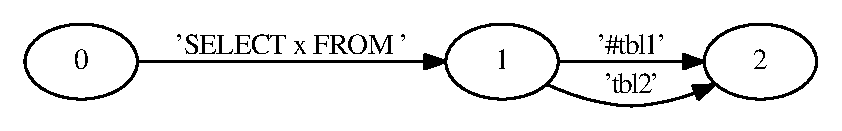
\includegraphics[scale=0.5]{Graphs/simpleSQL.eps}
    \end{center}
    \caption{Approximation for code presented in example above}
    \label{inp0}
\end{figure}

Next step~---~{\it abstract lexical analysis}~---~is a procedure which transforms input graph with string labels on edges into graph with token labels on edges. The result of input graph tokenization (or abstract lexing) is presented in the figure~\ref{inp0tok}. 

\begin{figure}[h!]
    \begin{center}
        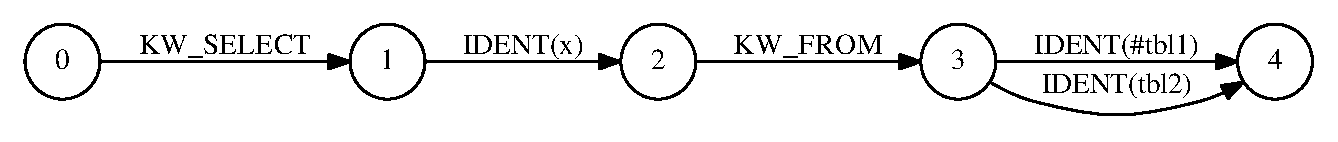
\includegraphics[scale=0.3]{Graphs/simple_sql.eps}
    \end{center}
    \caption{Result of tokenezation of graph in figure~\ref{inp0}}
    \label{inp0tok}
\end{figure}

Then we should perform {\it abstract parsing}. We use the second approach~---~reusing of classical LR parsing mechanism. Let we introduce the next example to explain basic ideas of abstract parsing. We will use the following grammar:

\begin{verbatim}
[<Start>]
s -> Ae
e -> BD | CD
\end{verbatim}

Input for analyzer builded by given grammar is a graph presented in the figure~\ref{inp1}.

\begin{figure}[h!]
    \begin{center}
        \includegraphics[scale=0.5]{Graphs/simple_grammar_input.eps}
    \end{center}
    \caption{Input graph to processing}
    \label{inp1}
\end{figure}

The set of parser states are computed for each graph vertice during parsing. All states that may be computed during parsing of all paths from start vertice to current should be computed for each vertice (figure~\ref{states}). For example, there are two different states for vertice 2 in the figure~\ref{states}: $\{e \to B.D; e \to C.D\}$. It is a result of sequences $AB$ and $AC$ parsing. 

\begin{figure}[h!]
    \begin{center}
        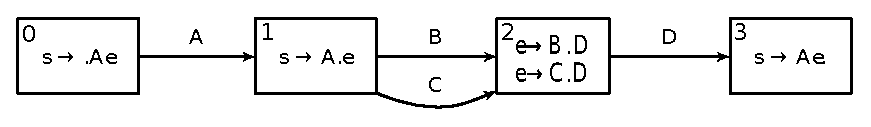
\includegraphics[scale=0.5]{Graphs/simple_grammar_items.eps}
    \end{center}
    \caption{Parser states for graph presented in figure ~\ref{inp1}}
    \label{states}
\end{figure}

Since the base of abstract parsing is classical LR algorithm, it is possible to process attributed grammars and, as a result, calculate user semantic actions.

\section{Generalized LR parsing}

Not all grammars are unambiguous but it is still necessary to process them, so there is a class of Generalized LR-analysis algorithms for ambiguous grammars handling. Classical GLR was introduced by Tomita~\cite{Tomita}. It is based on classical LR analysis~\cite{Grune} and has the number of significant differences making it possible to process ambiguous grammars. The algorithm uses parse tables, that are similar to parse tables for classical LR-algorithm, but can contain more than one possible action in each cell. This situation is named conflict and one of the two possible types can occur: {\it Shift/Reduce}~---~it is possible either to shift one more token from input stream or to reduce the stack~---~and {\it Reduce/Reduce}~---~there are more than one possibility to reduce the stack. In addition, more complex data structure~---~{\bf Graph Structured Stack, GSS}~\cite{Tomita}~---~is used instead of common stack. Manipulation with GSS is based on breadth-first traversal, so there are levels corresponding to the token position in the input stream.

Since it is possible to get more than one result of parsing in case of processing of ambiguous grammar then a special structure that allows to reuse nodes in parsing forest is used. This structure is introduced by Reker~\cite{SPPF} and named {\bf Shared Packed Parsing Forest} or {\bf SPPF}. SPPF is an inner data structure and it stores the forest data very compact. User defined semantic possibly requiring a lot of memory can be calculated after parsing finished only for necessary trees extracted from SPPF. This way we can reduce resource requirements. In our algorithm we also use classical GSS and SPPF as base data structures.

However, classical Tomita GLR constraints grammar. Elizabeth Scott et al.~\cite{RNGLR} proposed development of Tomita's idea~---~RNGLR-algorithm of syntactic analysis, which we use as a base for our algorithm. RNGLR-algorithm can handle arbitrary ambiguous grammar, like classical GLR-algorithm, and uses GSS and SPPF. The authors also introduced {\it push operation} instead of classical {\it shift} and {\it goto} which better correspond to adding new edges to GSS~\cite{RNGLR}. So {\bf Push(k)} is an action noting that symbol $k$ should be placed to stack. We will use this terminology for the rest part of the paper.

\section{Abstract Generalized LR Parsing}
\subsection{Input Data Format}

We approximate dynamic expression value set by constant propagation. Resulting data structure is a graph, which contains strings, used for expression construction, on its edges and its vertices correspond to concatenations. One might say we build finite automaton describing the language which consists of dynamically generated expression values.
	
If there is loops used in the construction of expression, value set may become infinite. We replace cycles in the graph with {\it single repetition} of its body for now. So the input data structure for our algorithm is {\bf Direct Acyclic Graph (DAG)} with only one source and sink vertices. This guarantee the finiteness of value set, but adversely affect on the reliability of the results since this replacement can lead to both loss of some possible expression and generation of new expressions. Let consider the following example. Suppose we need to process the code below.

\begin{verbatim}
1 query = "select * from ";
2 for(int i = 0; i < tables.size(); i++)
3 {
4    if(i != 0) query += ", ";
5    query += tables.get(i);
6 }
7 query += ";";
\end{verbatim}

	Regular expression $”select * from ” \cdot ((,|\varepsilon)\{tables.get(i)\}|\varepsilon)^{\star} \cdot ”;”$ is built as a regular approximation of set of possible values of variable \verb|query|. Corresponding finite automaton is presented in the figure~\ref{fa}. Notice, that we do not provide the value of expression $\{tables.get(i)\}$ as it depends on constant propagation algorithm possibilities. In order to get rid of cycle we replace it with single repetition of its body. Graph presented in the figure~\ref{faApprox} is the result of the replacement for our example.



\begin{figure}[h!]
    \begin{center}
        \includegraphics[scale=0.5]{Graphs/cyclesOrig.eps}
    \end{center}
    \caption{Correct finite automaton (graph representation)}
    \label{fa}
\end{figure}


\begin{figure}[h!]
    \begin{center}
        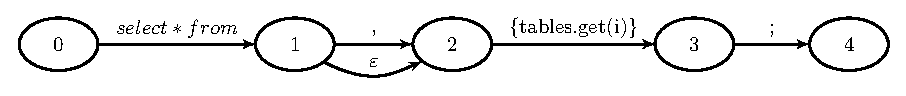
\includegraphics[scale=0.5]{Graphs/cyclesApproximation.eps}
    \end{center}
    \caption{Result of cycles approximation for graph in figure~\ref{fa}}
    \label{faApprox}
\end{figure}

As one can see, approximation graph does not contain paths corresponded to many values i.e. \verb|“select * from tbl1, tbl2;”| and \verb|“select * from;”|. This leads to impossibility of static check of theirs correctness. Only two possible values of initial infinite set can be generated from the approximation graph. Thus we cannot check all possible values in case of the loops that are used to construct queries. By the way, this approach provides enough data for such problems as code highlighting because all tokens which form expression will be processed. 

\subsection{Graph Structured Stack}

As soon as input data structure for our algorithm is DAG we can process all vertices in topological order instead of least-fixed point calculation. We define function $T(v)$ as a function which returns the number in topological order for vertex $v$. If there are more than one possible order, we choose one of them and fix it. 


Stack building in classical GLR is based on breadth-first traversal: firstly all actions with current level of stack should be performed, then if there are no available operation, pushes to the next level are performed. Operations in GLR stack are performed level-by-level. In RNGLR-algorithm levels correspond to input token number. We define level as a vertice number in topological order: this allows to avoid incorrect merging of stack branches. To process graph presented in the figure~\ref{inp2} we should process vertices sequentially in the next order: $0, 1, 2, 3, 4, 5, 6, 7$. In the figure~\ref{toposort} you can see the graph to process (in figure~\ref{inp2}) the layout of which is changed according to level data.


\begin{figure}[h!]
    \begin{center}
        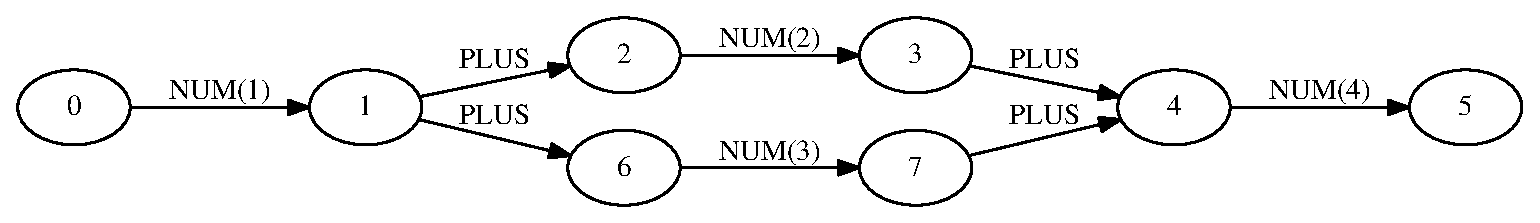
\includegraphics[scale=0.3]{Graphs/toposort0.eps}
    \end{center}
    \caption{Input graph for abstract parser}
    \label{inp2}
\end{figure}

\begin{figure}[h!]
    \begin{center}
        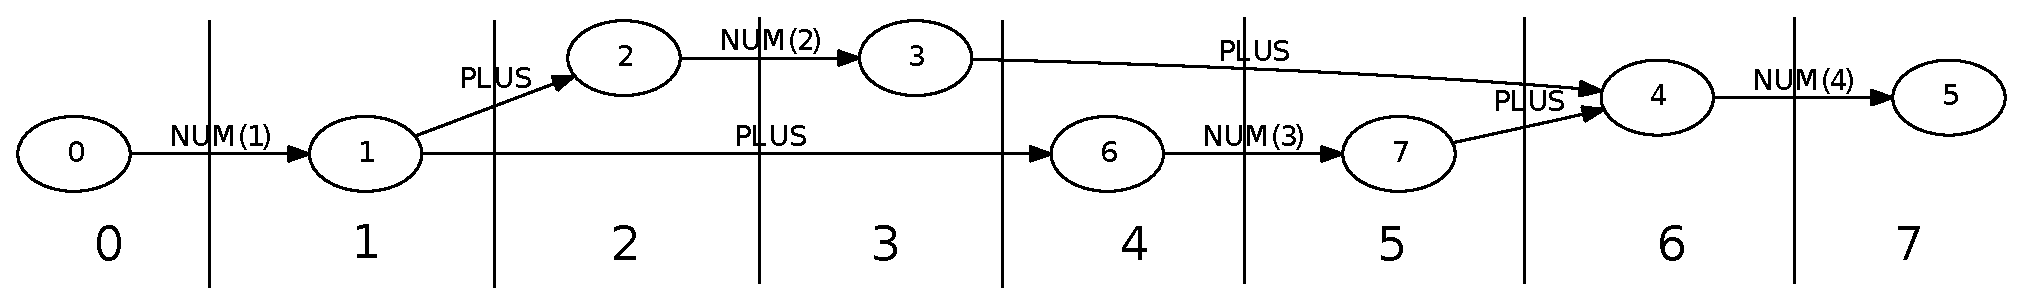
\includegraphics[scale=0.25]{Graphs/toposort1.eps}
    \end{center}
    \caption{Input graph in figure~\ref{inp2} with topological ordering applied}
    \label{toposort}
\end{figure}

Original GLR parsing algorithm can process {\it Shift/Reduce} and {\it Reduce/Reduce} conflicts~---~situations when available data are not enough to choose correct way of parsing continuation. GLR analyses every possible way in case of conflict. This allows to produce several derivations for single input sequence. One may notice that processing of the linear subgraph does not differ from the processing of sequential input. In vertices with more than one outgoing edges the situation is similar to the classical LR conflict: there are several possibilities to shift next token. This situation is not a conflict: all variants should be processed and there is no need to choose one of them, but we name this situation {\bf Shift/Shift} conflict by the analogy with classical conflicts. {\it Shift/Shift} conflict processing produces new branches in stack as any classical conflict, so forks in input graph correspond to forks in GSS. We improve original parsing algorithm with {\it Shift/Shift} conflict processing mechanism and it will be described below in details. 

GSS branch merging mechanism can be fully reused from GLR-algorithm. Vertices from graph are processed in the topological order. This ensures that states merging is possible only in~top vertices corresponded to branches which are produced by classical LR conflicts or in vertices with more than one incoming edges. In~both situations context and position in input data structure are the~same for processed vertices. If parsing states for any two vertices are equal, they can be merged by the analogy with GLR algorithm. Note that not all vertices with more than one incoming edges should initiate stack branches merging. 

The next difference from classical GSS manipulation is {\it push} operation introduced as a replacement of {\it goto} and {\it shift} operations. {\it Push} operation performs actual attachment of new edges to top vertices in GSS. In case of {\it Shift/Shift} conflict we should process every outgoing edge for the~vertice being processed. But only one of the~edges should be really added to GSS at a time: the edge $e$ with the minimal end number in the topological order {\it T(e.ToVertex)}. Remaining pushes should be postponed and applied only when {\it T(e.ToVertex)}~---~where $e$ is corresponded edge from input graph~---~is minimal for all vertices that are available to be processed during current step. This way we can avoid an early attachment of vertices, breaking topological order, to GSS. So, we do not perform all possible pushes like RNGLR and attach new edges only when it is necessary. 

\subsection{Example of GSS Construction}

We introduce the next example to demonstrate GSS manipulation in abstract parsing. We consider the following grammar of arithmetic expressions. Only two binary operators are specified: \ $+$ \ and \ $*$ \. The list of tokens is presented below.

\begin{verbatim}
PLUS = ‘+’
MULT = ‘*’
LBR = ‘(’
RBR = ‘)’
NUM = [1..9]
\end{verbatim}

And the final grammar is:

\begin{verbatim}
s -> s PLUS e | e
e -> e MULT t | t
t -> LBR s RBR
t -> NUM
\end{verbatim}

Input graph to be processed is presented in the figure~\ref{input}. This graph is ready for parsing: vertices are numbered in the topological order and edge labels are tokens. This graph is a representation of the following set of arithmetic expressions:

\begin{equation*}
%\begin{split}
\begin{array}{l}
\{ \\
1+4*(7*8)\ \\ \quad [0 \to 1 \to 2 \to 3 \to 8 \to 9 \to 10 \to 11 \to 12 \to 13] \\
1*5+(7*8)\ \\ \quad [0 \to 1 \to 4 \to 5 \to 8 \to 9 \to 10 \to 11 \to 12 \to 13] \\
1+6+(7*8)\ \\ \quad [0 \to 1 \to 6 \to 7 \to 8 \to 9 \to 10 \to 11 \to 12 \to 13] \\
\}
%\end{split}
\end{array}
\end{equation*}

\begin{figure*}
    \begin{center}
        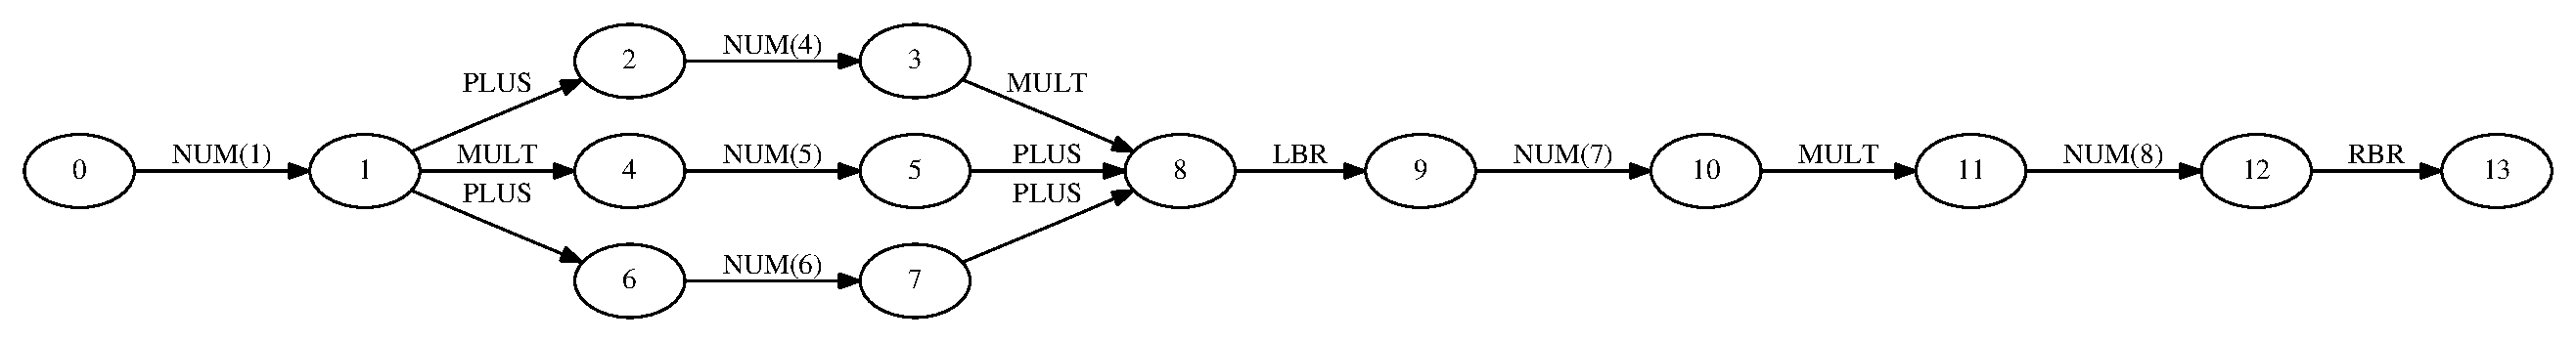
\includegraphics[scale=0.4]{Graphs/input1.eps}
    \end{center}
    \caption{Input graph GSS construction example}
    \label{input}
\end{figure*}

Now we can demonstrate stack transformations performed during analysis of the graph in the figure~\ref{input}. At the beginning stack contains one start vertice with number 0. At the first step token \verb|NUM| \ at the edge \ $ 0 \to 1$ \ is pushed. After that the sequence of reductions is performed. The reduction to nonterminal \verb|s| is final. Note that all intermediate outcome should be preserved in stack because pushes to next level may be available for every produced state. In our example token MULT at the edge \ $ 1 \to 4 $ \ can be pushed for state corresponded to vertex with \ $id=1$ \ and token \verb|PLUS| \ at the edges \ $1 \to 2$ \ and \ $1 \to 6$ \ can be pushed for state corresponded to vertex with $id=18$. On the other hand, there are no pushes for vertices with \ $id=21$ \ and \ $id=17$, so this vertices and outgoing edges will be removed at the next step. Stack after described operations is presented in the figure~\ref{stack1}.

\begin{figure}[h!]
    \begin{center}
        \includegraphics[scale=0.45]{Graphs/stack_1_2.eps}
    \end{center}
    \caption{GSS after first reduction to nonterminal {\it s} is finished}
    \label{stack1}
\end{figure}

At the next step we should process every outgoing edge for vertex with $id=1$ in the input graph. This vertex has three outgoing edges, so pushes for all of them should be constructed. But only one push should be available for further processing: corresponded to the vertex with minimal number. Postponed pushes will be processed in order of its start vertex topological number. In our example each branch will be processed sequentially until vertex with $id=8$ is processed. Then the next branch will be restored from postponed pushes and then processed. Stacks corresponded to processing of the paths \ $1 \to 2 \to 3 \to 8$ \ and \ $ 1 \to 4 \to 5 \to 8$ \  are presented in the figures~\ref{stack2}--\ref{stack4}. Note that in the figures~\ref{stack3}--\ref{stack7} postponed pushes are not drawn.

\begin{figure}[h!]
    \begin{center}
        \includegraphics[scale=0.45]{Graphs/stack_1_3_m.eps}
    \end{center}
    \caption{Stack with postponed pushes}
    \label{stack2}
\end{figure}

\begin{figure}[h!]
    \begin{center}
        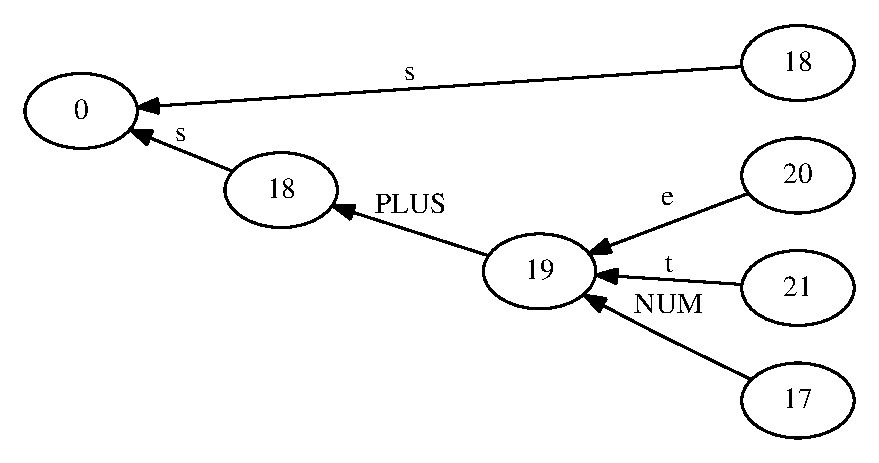
\includegraphics[scale=0.4]{Graphs/stack_1_4.eps}
    \end{center}
    \caption{Stack corresponded to processing of the path \\ \ $1 \to 2 \to 3$}
    \label{stack3}
\end{figure}

\begin{figure}[h!]
    \begin{center}
        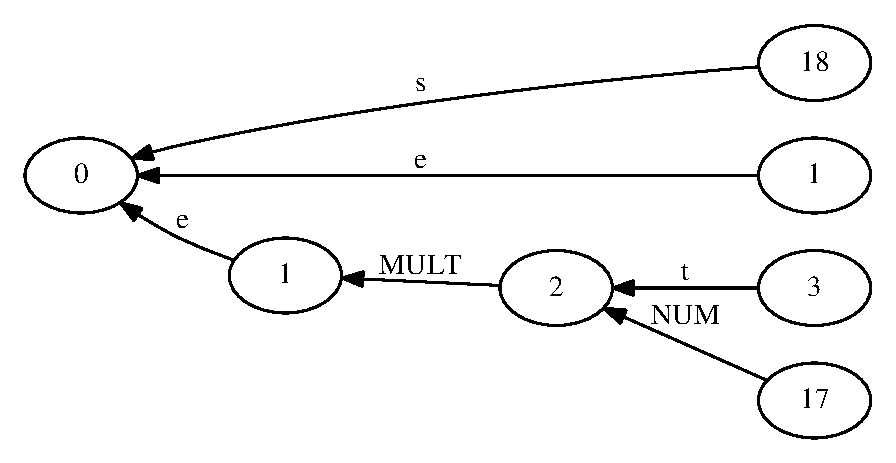
\includegraphics[scale=0.4]{Graphs/stack_1_6.eps}
    \end{center}
    \caption{Stack corresponded to processing of the path \\ \ $1 \to 4 \to 5$}
    \label{stack4}
\end{figure}

The stack presented in the figure~\ref{stack5} is got when all edges incoming to vertex with $id=8$ are processed. There are three incoming edges to vertex with $id=8$ \ but only two top vertices in stack are merged. It is happened because only two of them correspond to identical parsing states.  After that, when open brace form edge \ $8 \to 9$ \ in input graph is processed, all vertices corresponded to identical states and placed at the same level will be merged. Result of merge is presented in the figure~\ref{stack6}.

\begin{figure}[h!]
    \begin{center}
        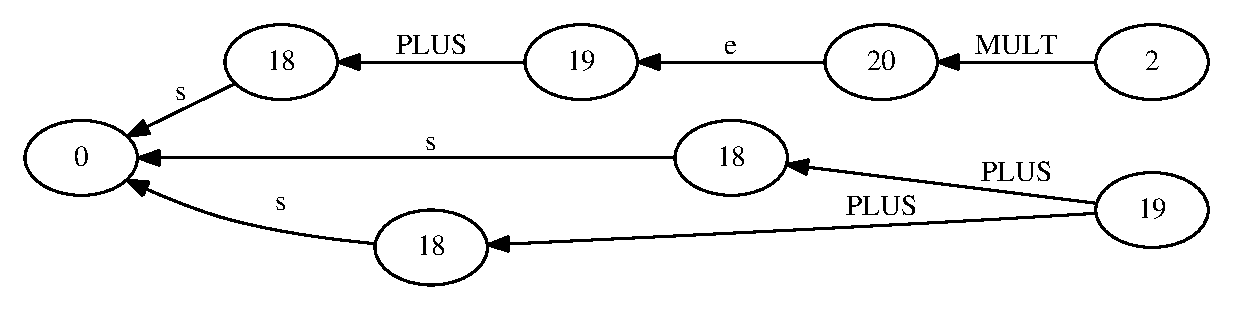
\includegraphics[scale=0.4]{Graphs/stack_4_9.eps}
    \end{center}
    \caption{GSS after all incoming edges to vertex with \ $id=8$ \ from the input graph are processed. Only two top vertices can be merged}
    \label{stack5}
\end{figure}

\begin{figure}[h!]
    \begin{center}
        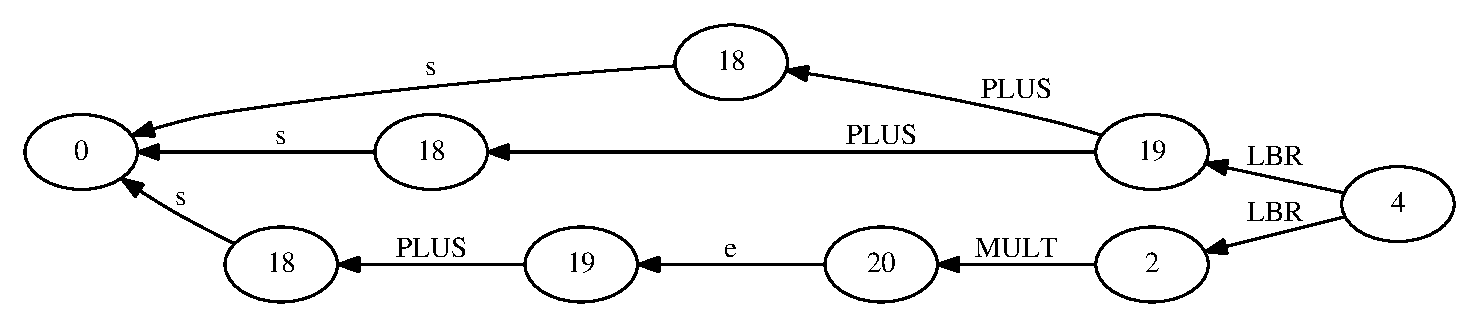
\includegraphics[scale=0.35]{Graphs/stack_4_10.eps}
    \end{center}
    \caption{GSS after all incoming edges to vertex with \ $id=9$ \ from the input graph are processed. All states are merged}
    \label{stack6}
\end{figure}

Further changes in the stack are performed in the order that has been described above. Final state of GSS is presented in the figure~\ref{stack7}.

\begin{figure*}
    \begin{center}
        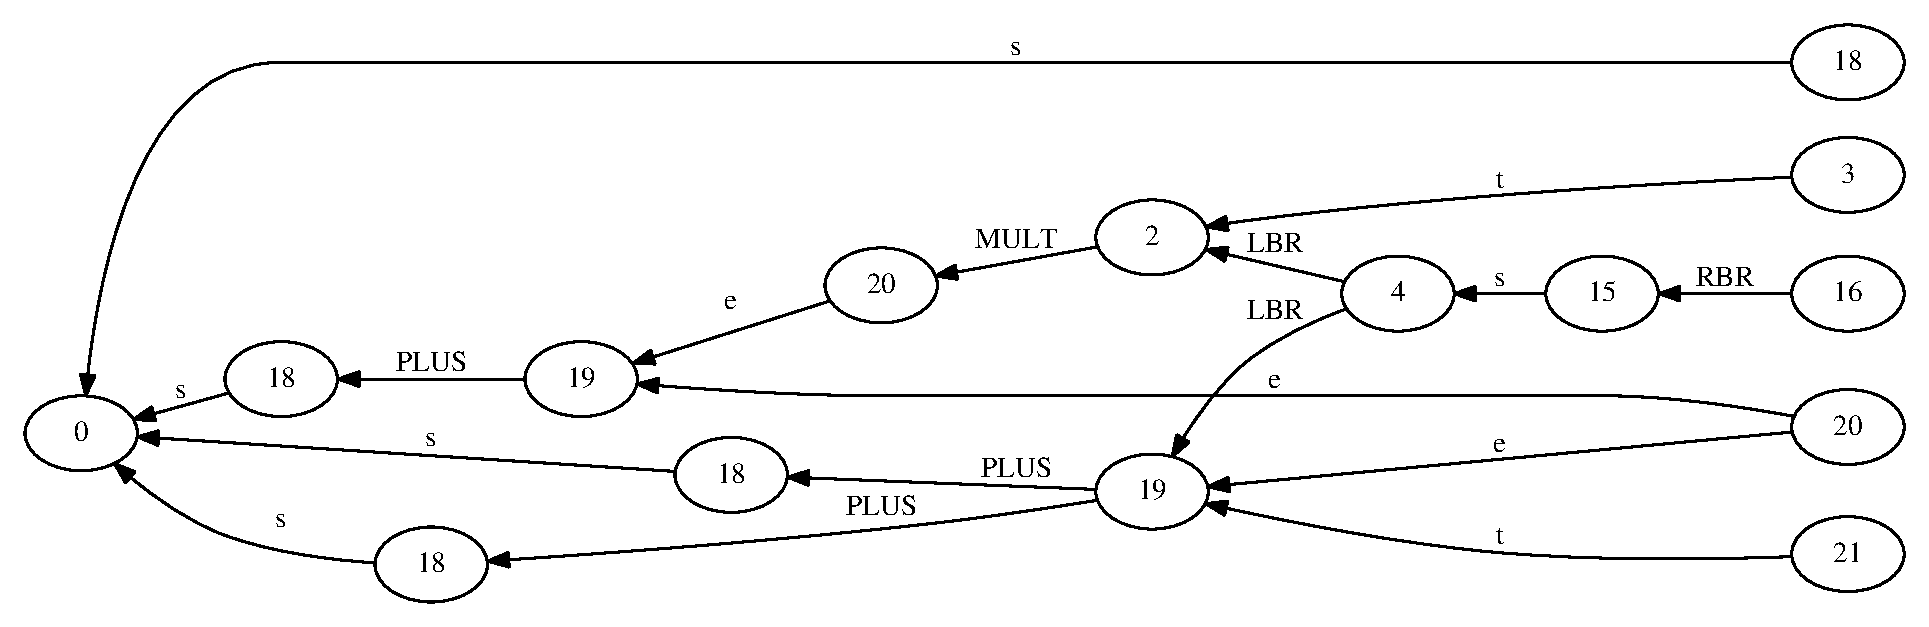
\includegraphics[scale=0.5]{Graphs/stack_5_13.eps}
    \end{center}
    \caption{Final GSS state for input graph in figure~\ref{input} }
    \label{stack7}
\end{figure*}

	We have demonstrated main steps of GSS construction: branching, pushes processing, branches merging. One can notice that it is similar to classical GLR GSS construction but differs in push processing.  


\subsection{Shared Packed Parsing Forest}

	Lightweight inner representation of parsing results~---~Shared Packed Parse Forest, SPPF~---~was proposed in a paper~\cite{SPPF} in order to minimize the size of parsing forest. After parsing completion SPPF can be used for semantic calculation or transformations. User can pick single parsing tree and calculate semantics only for it that can help to get rid of redundant calculation. Part of the calculation can also become redundant if it took place in the erroneous stack branch. These features are very valuable for abstract analysis as the number of common nodes in parse trees is huge and such nodes can be reused among the trees that are corresponded to different paths in input graph. The number of mistakes can also be enormous and there is no need to calculate semantics for the whole parse forest. Use of SPPF can significantly speed the abstract analysis up and reduce memory consumption. 

SPPF building in the process of abstract analysis does not differ from the one in RNGLR-algorithm. Intermediate nodes are introduced for correct representation of multiple possible parse trees for nonterminal that is processed. In our algorithm if there are several ways to construct node for nonterminal $s$, then additional vertices are created as children of this node and each of them is a root of parse tree for one of the possibilities. We paint nodes for such nonterminals in red in our figures.  You can see root node $s$ which has three different derivation (and thus three different parse trees merged into SPPF) in the figure~\ref{sppf}. Child nodes of the node $s$ with label $prod0$ are additional nodes. Their subtrees are corresponded to possible variants of $s$ derivation. 

As the process of SPPF construction is the same as in classic RNGLR-algorithm, we just provide the result for the example which has been described above.

\begin{figure}[h!]
    \begin{center}
        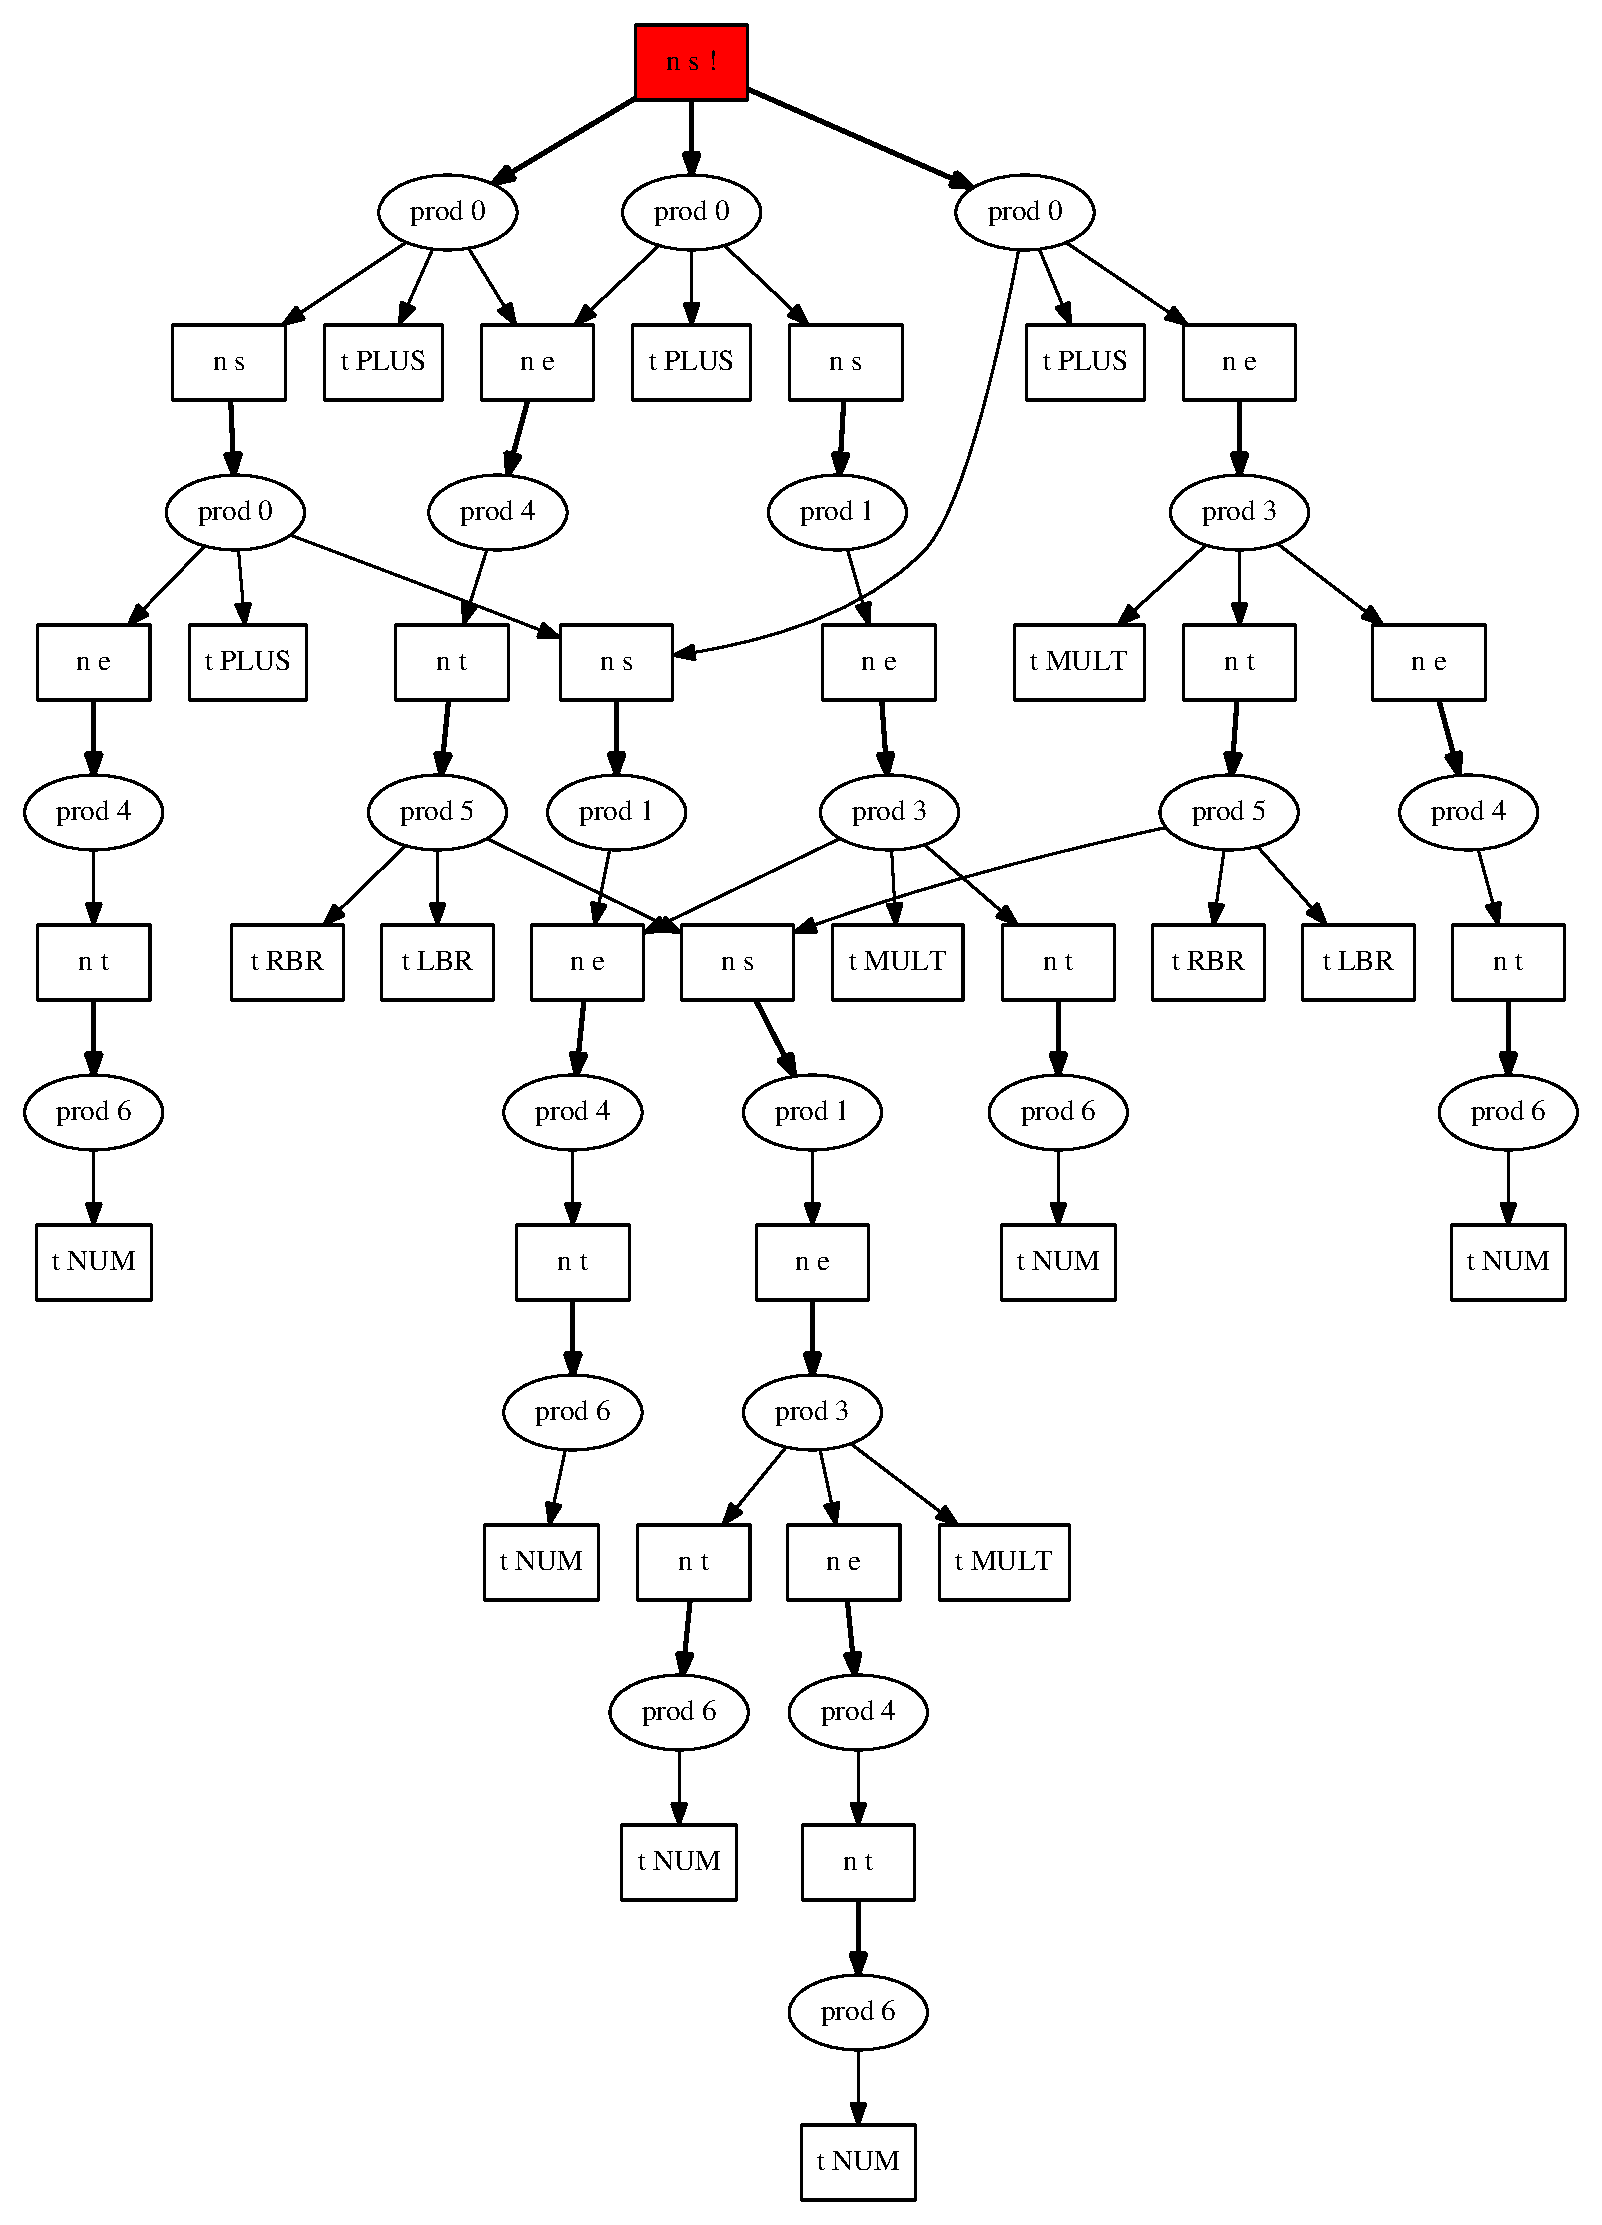
\includegraphics[scale=0.3]{Graphs/ast.eps}
    \end{center}
    \caption{SPPF for input presented in figure~\ref{input}.}
    \label{sppf}
\end{figure}

As it is said before, sometimes there is no need to calculate the semantics for the whole parse forest, or the forest is too large. It is also possible that there are trees which are correct syntactically but not semantically. In these cases lazy tree generation helps to avoid unnecessary semantic calculation. This way one can retrieve trees from SPPF and calculate semantics for them one-by-one.  

\subsection{Parsing Tables}

Abstract parsing uses original LR parsing tables. Kyung-Goo Doh, Hyunha Kim and David A. Schmid~\cite{AbstrParsing} use LALR(1) tables generated with ocamlyacc\footnote{Parser generator for OCaml. Project site (accessed: 01.07.2014): \url{http://caml.inria.fr/pub/docs/manual-ocaml-400/manual026.html}} in their work. We use RNGLR parsing algorithm  in our tool. RNGLR can process arbitrary context free grammars and has been proposed by Elizabeth Scott and Adrian Johnstone~\cite{RNGLR}. This algorithm has been implemented as a part of research project  
YaccConstructor\footnote{YaccConstructor is a platform for grammarware research and development. Project cite (accessed: 01.07.2014): \url{https://code.google.com/p/recursive-ascent/}}~\cite{GrigorevKirilenkoYC}. Different dialects of SQL with procedure extensions, JavaScript or other languages can play the role of embedded languages. Available specifications of this languages are often not LALR(1) and contain ambiguity. This makes it important to be able to process arbitrary context-free grammars in order to simplify development and support language processing tools. Therefore usage of GLR parsing algorithm instead of LALR(1) is better and our abstract parsing algorithm uses original RNGLR parsing tables. 



\section{Evaluation}

Generator of abstract parsers based on described parsing algorithm was implemented in F\#~\cite{FS} programming language as a part of YaccConstructor. RNGLR parser generator used as a base of our algorithm was implemented before as a part of YaccConstructor. As we discussed before, the~generator itself is reused without any changes. Table interpreter was modified, although main data structures and base logic were reused. One can use an implemented framework for generation of a tool designed for abstract parsing of the language that is specified in an input grammar. Thus the framework is similar to the classical parser generators. Abstract lexer generator and approximation builder were also implemented. General high-level structure of our tool is presented in the figure~\ref{tStruct}.

\begin{figure*}%[h!]
    \begin{center}
        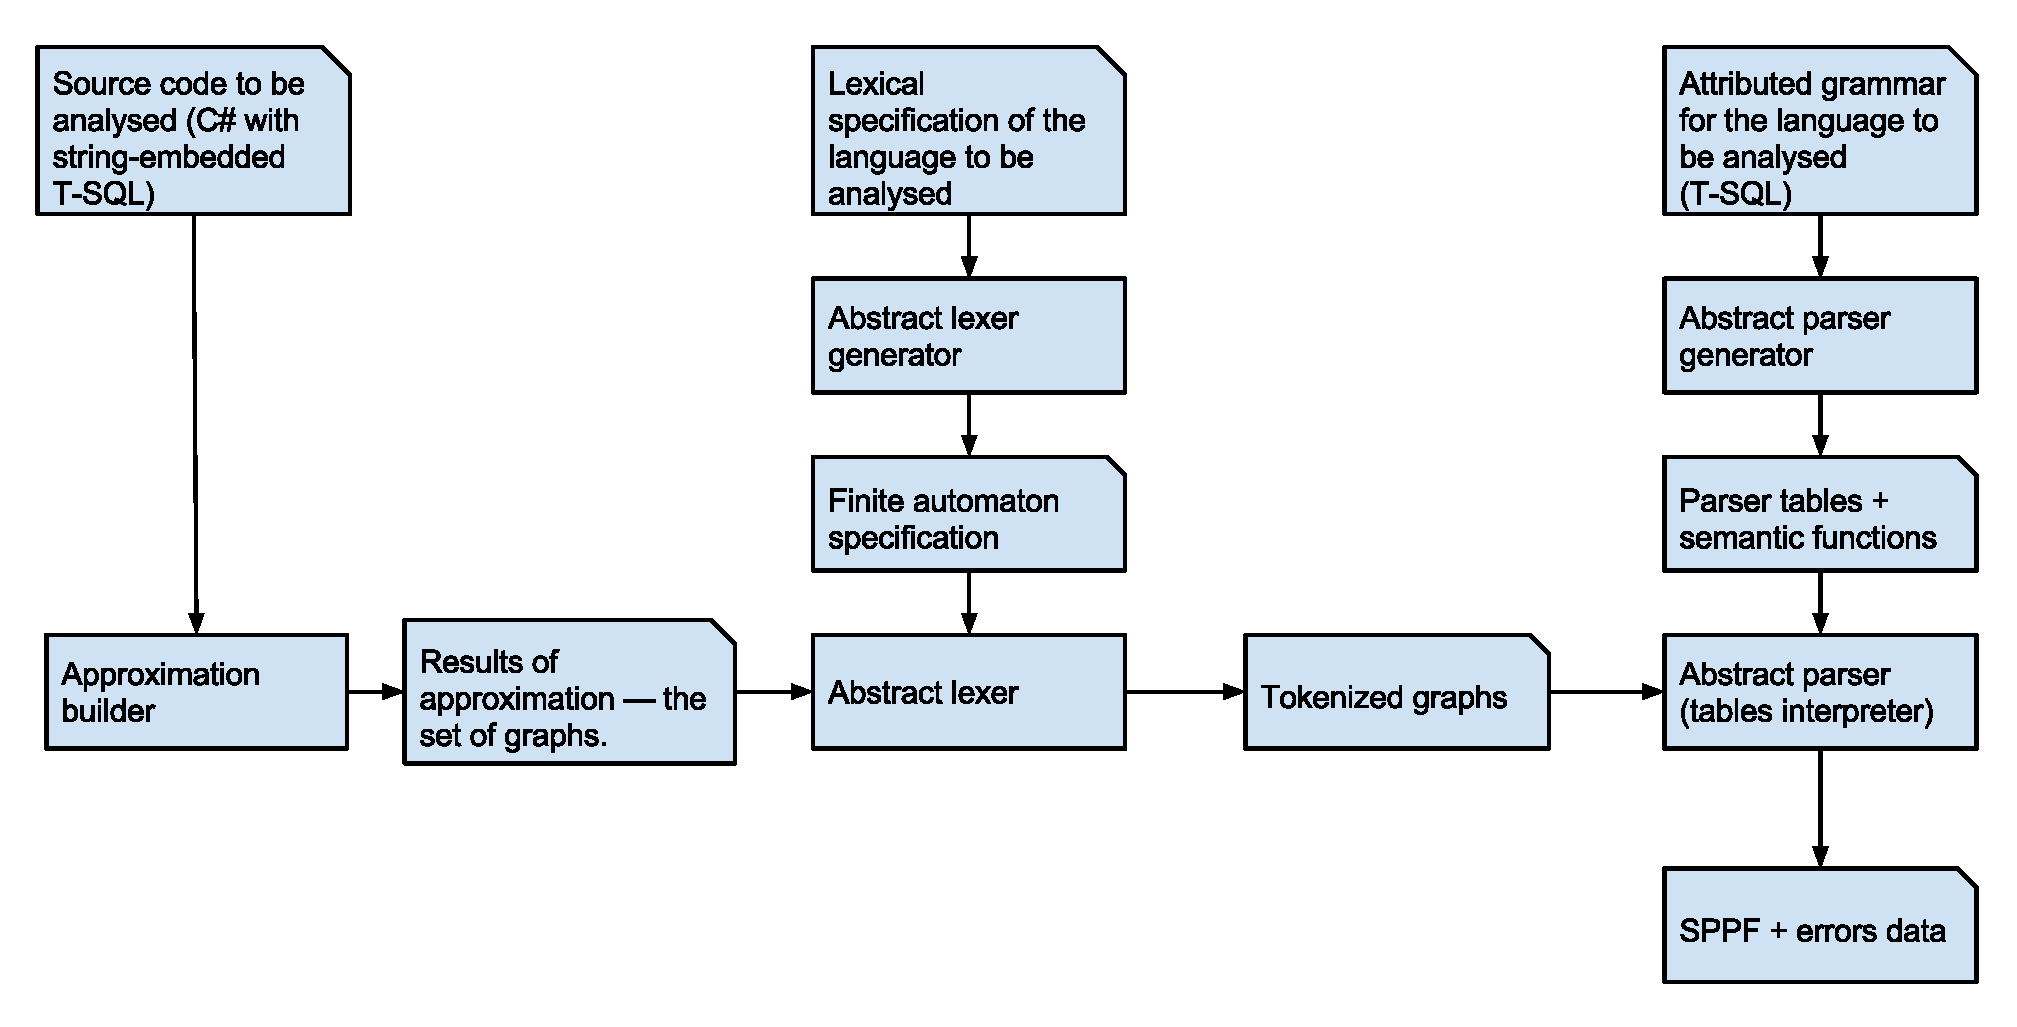
\includegraphics[scale=0.5]{Graphs/General_structure_of_generator.eps}
    \end{center}
    \caption{Abstract analysis tool structure}
    \label{tStruct}
\end{figure*}

We has compared generated parser with similar tools to evaluate its performance. Only Alvor\footnote{Repository of Alvor (accessed: 01.07.2014) \url{https://code.google.com/p/alvor/}} is available for comparison at this moment. Tool developed by Kyung-Goo Doh et al. and described in their papers is also very important for comparison but neither sources nor binaries of the tool are available.

Grammar of the subset of Transact SQL language was developed for  testing purposes. Grammar contains specification for procedure extension and Data Manipulation Language. The grammar developed is available in a project repository\footnote{Repository of YaccConstructor (accessed: 01.07.2014) \url{https://code.google.com/p/recursive-ascent/}}. We aimed to test parser only so approximation step was omitted. An input data is a set of previously generated and serialized representations of dynamic expression approximations. We use our experience in production information system migration  from MS-SQL Server 2005 to Oracle 11gR2 to generate relevant input data~\cite{GrigorevDSQL}. The source system consists of 850 stored procedures and contains more than 3000 dynamic queries. Total size of migrated system is 2.7 million lines of code. The number of operations used to construct values for more than half of queries is between 7 and 212, average is 40. We performed an information system source code analysis and figured out that the most frequent template for dynamic query building is sequential concatenation of blocks constructed with branching operators: {\it if} statement or {\it case} statement. Input data for tests were generated according to this result. Each test is described by two parameters: the number of parallel edges in each block $m$, and the number of sequentially concatenated blocks $n$. All blocks in one sequence have equal number of parallel edges. Example of graph with $m = 3$ and $n = 2$ is presented in the figure~\ref{nmExample}.

\begin{figure}[h!]
    \begin{center}
        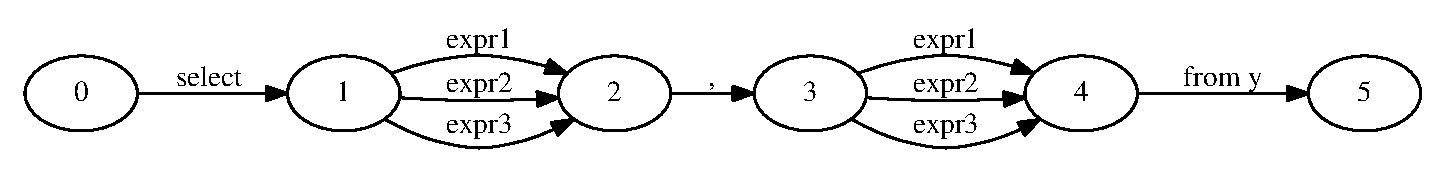
\includegraphics[scale=0.35]{Graphs/x_10.eps}
    \end{center}
    \caption{Example of input graph for $n=2$ and $m=3$}
    \label{nmExample}
\end{figure}

Structure of input data was identical for all tested tools but representation of data is different and we should apply it in test generator. YaccConstructor uses graph as an input data structure and loads data from DOT\footnote{DOT is a text language for graph description. Language specification (accessed: 01.07.2014): \url{http://www.graphviz.org/doc/info/lang.html}} file. On the other hand, Alvor uses regular expression corresponded to finite automaton which was represented as a graph for YaccConstructor and loads it from text file. The following constructions are available:

\begin{itemize}
\item "a" "b"~---~concatenation
\item  \{"a", "b", "c"\}~---~variants
\end{itemize}

	We created a test set generator which takes patterns as an input and generates tests using this pattern for both YaccConstructor and Alvor. Input regular expression for Alvor and the equivalent input graph for YaccConstructor are presented in the figure~\ref{YCAlvor}.

\begin{figure}[h!]
    \begin{center}
        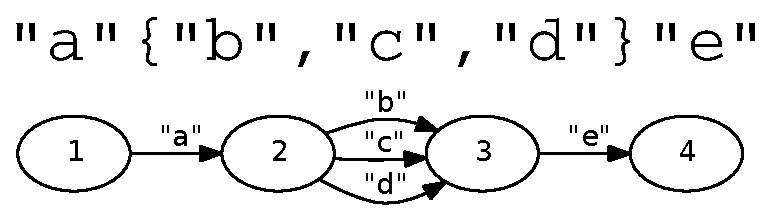
\includegraphics[scale=0.5]{Graphs/YcAlvorInput.eps}
    \end{center}
    \caption{Eqivalent input for YaccConstructor and Alvor}
    \label{YCAlvor}
\end{figure}


We used PC with the next configuration for test purposes.

\begin{itemize}
    \item Operation system: Windows 8.1 Pro
    \item Operation system type: 64-bit OS, x64-based CPU
    \item CPU: Intel Core i7-2620M CPU 2.70GHz
    \item RAM: 12Gb
    \item Tools were implemented for different platforms (Alvor for Java platform, YaccConstructor for .Net framework) so we used corresponding environments:
        \begin{itemize}
        \item Java: 
            \begin{itemize}
                \item Java(TM) SE Runtime Environment (build 1.7.0\_45-b18)
                \item Java HotSpot(TM) 64-Bit Server VM (build 24.45-b08, mixed mode)
            \end{itemize}
        \item .Net:
            \begin{itemize}
                \item Microsoft.NET Framrwork v4.0.30319                
            \end{itemize}
        \end{itemize}
\end{itemize}

You can find the set of diagrams which illustrates the result of performance measurement for YaccConstructor and Alvor (figures ~\ref{perfm1}, ~\ref{perfm2}, ~\ref{perfm3}, and~\ref{performance}). Tools were tested for input data generated with template described above. Values of $m$ \ is between 1 and 5, and $n$ \ is up to 200.


%\begin{figure*}
    %\begin{center}
      \begin{figure}[h!]%{0.33\textwidth}
        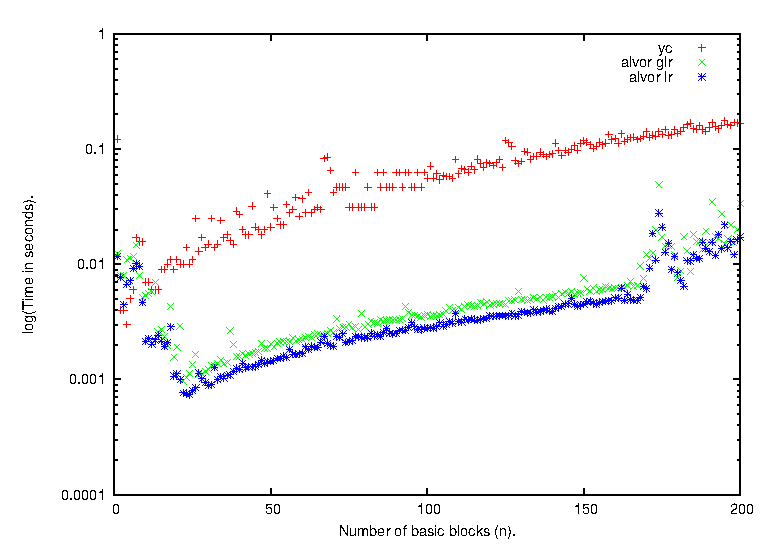
\includegraphics[scale=0.65]{Graphics/m1.eps}
        \caption{Performance comparison of YaccConstructor and Alvor for $m = 1$}
        \label{perfm1}
      \end{figure}
      %~
      \begin{figure}[h!]%{0.33\textwidth}
        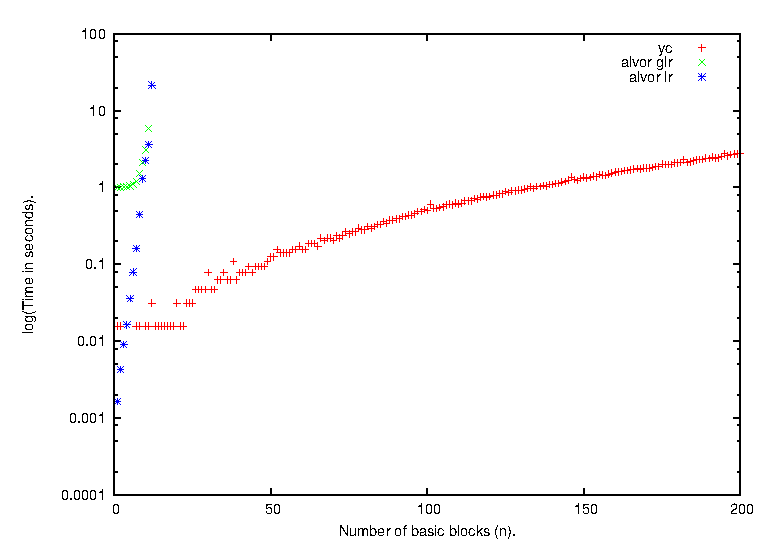
\includegraphics[scale=0.65]{Graphics/m2.eps}
        \caption{Performance comparison of YaccConstructor and Alvor for $m = 2$}
        \label{perfm2}
      \end{figure}
      %~
      \begin{figure}[h!]%{0.33\textwidth}
        \includegraphics[scale=0.65]{Graphics/m3.eps}
        \caption{Performance comparison of YaccConstructor and Alvor for $m = 3$}
       \label{perfm3}
      \end{figure}    
    %\end{center}
    %\caption{Performance comparison of YaccComctructor and Alvor}
    %\label{performance}
%\end{figure*}

\begin{figure*}
	\begin{center}
      \begin{subfigure}[b]{0.45\textwidth}
        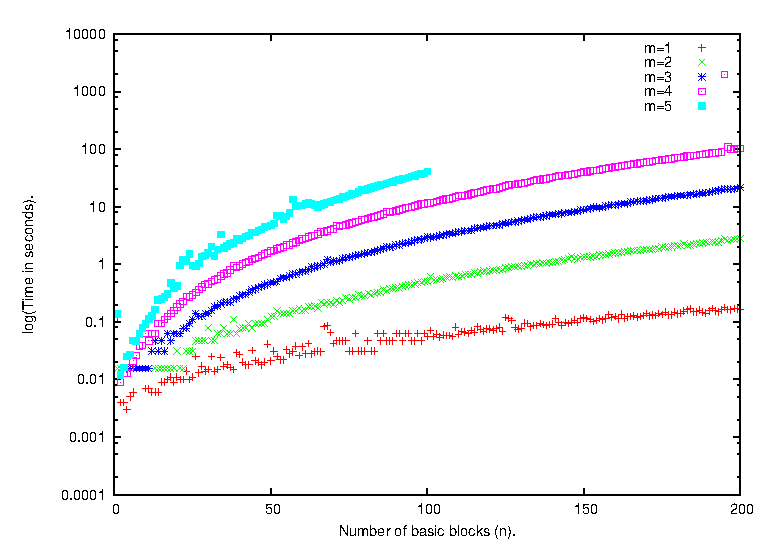
\includegraphics[scale=0.65]{Graphics/yc.eps}
        \caption{Performance of YaccConstructor for $m \in \{1; 2;3;4;5\}$}
       \label{perfYC}
      \end{subfigure}
      ~
      \begin{subfigure}[b]{0.45\textwidth}
        \includegraphics[scale=0.65]{Graphics/alvor.eps}
        \caption{Performance of Alvor for $m \in \{1; 2;3;4;5\}$}
       \label{perfAlvor}
      \end{subfigure}
    
    \end{center}
    \caption{Performance comparison of YaccComctructor and Alvor}
    \label{performance}
\end{figure*}

Note that we stopped the measurements for Alvor after very small value of $n$ because it required more than 4Gb of RAM and took much execution time. It seems that Alvor requires exponential resources to process an input with big number of branches. It can be caused by the fact that Alvor can only branch stack and does not perform the merging.


From the data gathered it can be concluded that the performance of implemented tool is better than performance of Alvor in a wide rage of practical cases: 2--3 parallel edges in block and the number of blocks up to 200. But in case of linear input our tool performance is worse than Alvor performance.

\section{Future Work}

One of the main application of developed tool is error detecting, so it is important to improve corresponded algorithms. Error reporting and error recovery in generalized LR parsing are nontrivial problems. A considerable amount of research has been done on improving error reporting for LR parsers, although relatively little work has been done for GLR parsers~\cite{GLROverview}. During the experiments we figured out that error processing in GLR-based abstract parsing is far more complex than in classical GLR parsing algorithm. It is caused by increased algorithm complexity. On the other hand, error processing in LL parsing algorithm is easier than in LR-algorithm, so we are going to investigate GLL parsing algorithm~\cite{GLL} and research whether it can be used as a base for abstract parsing algorithm. We expect that GLL-based abstract parsing will be based on the same ideas as GLR-based algorithm because it also manipulates with GSS and SPPF data structures. We also expect error processing in GLL-based abstract parsing to be more qualitative.

The situations in which there are huge amount of code which contains a few errors and should be processed in short time often occur in software reengineering. In this case GLR-based abstract parsing algorithm may be useful in spite of error processing issues. It is important that in such case we may notify developers of every suspicious situation in code. Migration to generalized parsing algorithms with better performance than RNGLR~---~BRNGLR~\cite{BRNGLR} or RIGLR~\cite{RIGLR}~---~ may help to increase performance of abstract parsing.

It is also important to improve quality of analysis so the next big problem is improvement and adjustment of approximation. Firstly, it is necessary to support cycles in input graph, but this may provoke parsing complexity increase and performance problems. As a possible solution to this problems, improved algorithm should only be applied when it is necessary (input graph contains cycles). %Our current experience of processing of real world information systems shows that cycles are not very popular in dynamic expressions construction.



%\appendix
%\section{Appendix Title}

%This is the text of the appendix, if you need one.

%\acks

%Acknowledgments, if needed.

% We recommend abbrvnat bibliography style.

\bibliographystyle{abbrvnat}

% The bibliography should be embedded for final submission.
%ALVOR1, LRAbstrParsing, Minamide, StringExpr, SAofStrVal, SAForInject, Dasgupta

\begin{thebibliography}{}
\softraggedright

\bibitem{ALVOR1}
Annamaa A., Breslav A., Kabanov J. e.a. An Interactive Tool for Analyzing Embedded SQL Queries. Programming Languages and Systems. LNCS, vol. 6461. Springer: Berlin; Heidelberg, p. 131--138, 2010.

\bibitem{ALVOR2}
Annamaa A., Breslav A., Vene V. Using Abstract Lexical Analysis and Parsing to Detect Errors in String-embedded DSL Statements, Proceedings of the 22nd Nordic Workshop on Programming Theory. Marina Walden and Luigia Petre, editors, p. 20--22. 2010.

\bibitem{AbstrParsing}
Kyung-Goo Doh, Hyunha Kim, David A. Schmidt. Abstract Parsing: Static Analysis of Dynamically Generated Sring Output Using LR-parsing Technology, Proceedings of the 16th International Symposium on Static Analysis, SAS’09. Springer-Verlag: Berlin; Heidelberg, p. 256--272, 2009.

\bibitem{LRAbstrParsing}
Kyung-Goo Doh, Hyunha Kim, and David A. Schmidt. Abstract LR-parsing, In Formal modeling, Gul Agha, José Meseguer, and Olivier Danvy (Eds.). Springer-Verlag, Berlin, Heidelberg, p. 90--109, 2011.

\bibitem{LRAbstrParsingSema}
H. Kim, K. Doh,  and D.A. Schmidt,  Static Validation of Dynamically Generated HTML Documents Based on Abstract Parsing and Semantic Processing.  ;In Proceedings of SAS, 194 -- 214, 2013.

\bibitem{GLL}
Elizabeth Scott and Adrian Johnstone. 2010. GLL Parsing, Electron. Notes Theor. Comput. Sci. 253, 7 (September 2010), p. 177--189. 

\bibitem{SPPF}
Rekers J. G. 1992. Parser generation for interactive environments. Ph.D. thesis, Universty of Amsterdam.

\bibitem{Grune}
Grune D., Ceriel J. H. Jacobs. Parsing techniques: a practical guide. Ellis Horwood, Upper Saddle River, NJ, USA, 1990. p. 322.

\bibitem{GrigorevKirilenkoYC}
Iakov Kirilenko, Semen Grigorev, and Dmitriy Avdiukhin. Syntax analyzers development in automated reengineering of informational system.
St. Petersburg State Polytechnical University Journal. Computer Science. Telecommunications and Control Systems, 174(3), June 2013.

\bibitem{Minamide}
Yasuhiko Minamide. Static approximation of dynamically generated web pages. In Proceedings of the 14th International Conference on World
  Wide Web, WWW '05, p. 432--441, New York, NY, USA, 2005. ACM.

\bibitem{RNGLR}
Elizabeth Scott and Adrian Johnstone. Right nulled glr parsers. ACM Trans. Program. Lang. Syst., 28(4):p. 577 -- 618, July 2006.

\bibitem{StringExpr}
Aske Simon Christensen, M{\o}ller A., Michael I. Schwartzbach. Precise analysis of string expressions, Proc. 10th International Static Analysis Symposium (SAS), Vol. 2694 of LNCS. Springer-Verlag: Berlin; Heidelberg, June, p. 1 -- 18, 2003.

\balance

\bibitem{SAofStrVal}
Costantini G., Ferrara P., Cortesi F. Static analysis of string values, Proceedings of the 13th international conference on Formal methods and software engineering, ICFEM’11. Springer-Verlag: Berlin; Heidelberg, p. 505-521, 2011.


\bibitem{ISO}
ISO. ISO/IEC 9075:1992: Title: Information technology~---~Database languages~---~SQL. 1992. p. 668.

\bibitem{SAForInject}
Xiang Fu, Xin Lu, Peltsverger B. e.a. A static analysis framework for detecting SQL injection vulnerabilities, Proceedings of the 31st Annual International Computer Software and Applications Conference. Vol. 01, COMPSAC’07, Washington, DC, USA, IEEE Computer Society, p. 87--96, 2007.

\bibitem{Dasgupta}
Arjun Dasgupta, Vivek Narasayya, and Manoj Syamala. A static analysis framework for database applications. In Proceedings of the 2009 IEEE International Conference on Data Engineering, ICDE '09, p. 1403--1414, Washington, DC, USA, 2009. IEEE Computer Society.

\bibitem{GrigorevDSQL}
Semen Grigorev. Automated transformation of dynamic sql queries in information system reengineering. Master's thesis, Saint-Petersburg State University, 2012.

\bibitem{GLROverview}
 Giorgios Robert Economopoulos. Generalised LR parsing algorithms. 2006.
 
\bibitem{Tomita} 
 Tomita, Masaru. LR parsers for natural languages, In 10th International Conference on Computational Linguistics, p. 354--357. ACL, 1984.

\bibitem{AbstractInterpretation} 
 Patrick Cousot and Radhia Cousot. 1977. Abstract interpretation: a unified lattice model for static analysis of programs by construction or approximation of fixpoints. In Proceedings of the 4th ACM SIGACT-SIGPLAN symposium on Principles of programming languages (POPL '77). ACM, New York, NY, USA, p. 238--252.
 
\bibitem{FS}
Syme D., Granicz A., and Cisternino A.: Expert F\#, Apress (2007).

\bibitem{BRNGLR}
Elizabeth Scott, Adrian Johnstone, and Rob Economopoulos. 2007. BRNGLR: a cubic Tomita-style GLR parsing algorithm. Acta Inf. 44, 6 (September 2007), p. 427-461.

\bibitem{RIGLR}
Elizabeth Scott and Adrian Johnstone. Table based parsers with reduced stack activity. Technical Report CSD-TR-02-08, Royal Holloway, University of London, Department of Computer Science, Egham, Surrey TW20 0EX, England, May 2003.

%\bibitem{DragonBook}
%Alfred V. Aho , Ravi Sethi , Jeffrey D. Ullman, Compilers: principles, techniques, and tools, Addison-Wesley Longman Publishing Co., Inc., Boston, MA, 1986

\end{thebibliography}



\end{document}
